\documentclass[10pt]{article}
\usepackage[letterpaper,margin=.65in]{geometry}
\usepackage{amsmath,amssymb}
\usepackage{figure-ink}
\pagestyle{empty}
\setlength{\parindent}{0pt}
\begin{document}
\begin{center}\Large Reproducible ink figures\end{center}
\small Fixed vector grain, exact coordinates, native Computer Modern labels.

\medskip\textbf{1. Upper-triangular map}\par
\begin{center}
\begin{tikzpicture}[font=\small]
\InkRegion[inkblue]{(-.7,-.45)--(4.9,-.45)--(5.8,2.65)--(.2,2.65)--cycle}
\InkStroke[inkblue!65]{(-.7,-.45)--(.2,2.65)--(5.8,2.65)}
\InkStroke[inkblue!65]{(-.7,-.45)--(4.9,-.45)--(5.8,2.65)}
\InkStroke[inkred]{(-.8,0)--(5.5,0)}
\InkStroke[ink arrow,inkred]{(0,0)--(3,0)}
\InkStroke[ink arrow]{(0,0)--(1,0)}
\InkStroke[ink guide,inkslate]{(1,1)--(2,2)}
\InkStroke[ink guide,inkamber,-{Stealth[length=4pt,width=1.8pt]},shorten >=4pt]{(2,2)--(4,2)}
\InkStroke[ink arrow,inkblue]{(0,0)--(4,2)}
\InkStroke[ink arrow]{(0,0)--(1,1)}
\fill (0,0) circle (.9pt);
\node[below left] at (0,0) {$0$};
\node[below] at (1,0) {$v_1$};\node[below,inkred] at (3,0) {$Tv_1$};
\node[above left] at (1,1) {$v_2$};
\node[above left,inkslate] at (2,2) {$2v_2$};
\node[above,inkamber] at (3,2) {$+2v_1$};
\node[right,inkblue] at (4,2) {$Tv_2$};
\node[below,inkred] at (5.4,0) {$U_1$};\node[inkblue] at (.7,2.35) {$U_2$};
\node[anchor=west] at (6.5,1.2) {$\displaystyle\mathcal M(T)=\begin{pmatrix}\textcolor{inkred}{3}&\textcolor{inkamber}{2}\\0&\textcolor{inkblue}{2}\end{pmatrix}$};
\end{tikzpicture}
\end{center}
$v_1=(1,0)$, $v_2=(1,1)$; hence $Tv_1=3v_1$ and $Tv_2=2v_1+2v_2$.
The parallelogram shows only a portion of the plane $U_2$.

\bigskip\textbf{2. Orthogonal projection}\par
\begin{center}
\begin{tikzpicture}[font=\small]
\InkRegion[inkblue]{(0,0)--(3,0)--(3,2)--cycle}
\InkStroke[inkslate]{(-.7,0)--(4.5,0)}
\InkStroke[ink arrow,inkblue]{(0,0)--(3,2)}
\InkStroke[ink arrow,inkgreen]{(0,0)--(3,0)}
\InkStroke[ink guide,inkred]{(3,0)--(3,2)}
\InkStroke[inkslate]{(2.8,0)--(2.8,.2)--(3,.2)}
\fill (0,0) circle (.9pt);
\node[below left] at (0,0) {$0$};\node[above right,inkblue] at (3,2) {$v=(3,2)$};
\node[below,inkgreen] at (2,0) {$p=(3,0)$};
\node[right,inkred] at (3,1) {$v-p=(0,2)$};\node[below] at (4.5,0) {$U$};
\node[anchor=west,align=left] at (6,1) {$p=\operatorname{proj}_U v$\\[5pt]$\langle p,v-p\rangle=0$};
\end{tikzpicture}
\end{center}
Here $U$ is the horizontal line. The shaded triangle marks the vector decomposition; it is not a subspace.

\bigskip\textbf{3. Counting nilpotent Jordan blocks}\par
\begin{center}
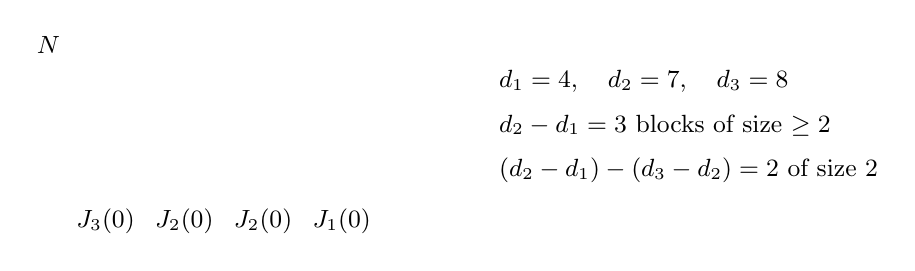
\begin{tikzpicture}[font=\small]
\foreach \x/\h in {0/3,1/2,2/2,3/1}{
 \foreach \y in {1,...,\h}{
  \ifnum\y=2 \def\cellink{inkblue}\else\def\cellink{inkslate}\fi
  \ifnum\y=3 \path[fill=white] (\x,\y*.55) rectangle ++(.65,.55);
  \else\InkRegion[\cellink]{(\x,\y*.55) rectangle ++(.65,.55)}\fi
  \InkStroke{(\x,\y*.55) rectangle ++(.65,.55)}
 }
 \node[below] at (\x+.325,.48) {$J_{\h}(0)$};
}
\InkStroke[ink arrow]{(-.4,2.2)--(-.4,.55)}\node[above] at (-.4,2.2) {$N$};
\node[anchor=west,align=left] at (5.2,1.4) {$d_1=4,\quad d_2=7,\quad d_3=8$\\[5pt]$d_2-d_1=3$ blocks of size $\geq2$\\[5pt]$(d_2-d_1)-(d_3-d_2)=2$ of size $2$};
\end{tikzpicture}
\end{center}
Here $d_k=\dim\operatorname{null}N^k$. Each cell represents one basis vector. $N$ moves down its column and sends the bottom cell to $0$.
\end{document}
